% !TEX root = ../report.tex

\clearpage
\chapter{Pattern Documentation}
\label{ch:patterns}


\section{Core}
\subsection{Layers}
% see https://www.docker.com/sites/default/files/what-is-vm-diagram.png

\subsection{Client-Server}
% see https://docs.docker.com/engine/introduction/understanding-docker/
% also nice image we can borrow: https://docs.docker.com/engine/article-img/architecture.svg
\begin{figure}[H]
\caption{An overview of the Docker architecture, showing the client and daemon. Source: \cite{dockerarchi}.}
\centering
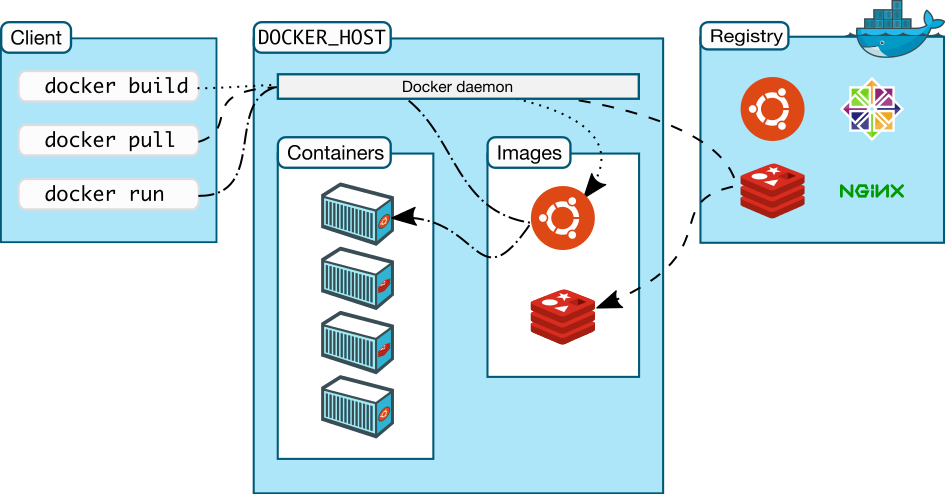
\includegraphics[scale=0.4]{4-softwarearch/images/architecture.png}
\end{figure}

\begin{description}
\item [Traceability]~\\
The Client-Server pattern can be deducted from the online documentation\cite{dockerarchi}.

\item [Source]~\\
Architectural patterns revisited -- a pattern language, P. 29 \cite{avgeriou2005architectural}

\item [Issue]~\\
%TODO: why did they choose this, just to connect to remote daemons or is it for seperation of concerns??
% it is possible to connect the docker client to a remote docker daemon.

\item [Assumptions/Constraints]~

\item [Solution]~\\
Docker uses a Client-Server architecture. The client, a binary supplying a command-line interface, act as the primary interface for the user. The user enters command into this client, which are then send to a server: the docker daemon. 

The daemon is a background process, which supplies the requested services to the client. The daemon exposes a REST interface.

For Docker, the client can be configured to connect to other daemon processes than the one running on the local machine. It can be configured to connect to remote Docker daemons as well, allowing the user to issue commands to daemons running remotely.

\item [Rationale] ~\\
Client-Server separates the interaction with the user from the actual domain logic and offers the flexibility needed to connect to remote daemons. %todo: make this sensible

\item [Implications]~\\


\item [Related Patterns]~\\


\end{description}

\subsection{Shared repository}
Can we consider the docker registry a shared repository?




\section{Modules}
\subsection{Interceptor}
\subsection{Plugin}

